% !TEX root = ../thesis.tex

\section{Network Architecture and Parameters}
\label{ch4:app:architecture}

Our thermodynamic map is parameterized as a score-based model using a U-net \cite{unet} with four Resnet downsampling blocks, followed by an attention layer, and four Resnet upsampling blocks. For all experiments, we use a learning rate of $10^{-3}$ with the Adam optimizer \cite{Adam}. We also employ self-conditioning to accelerate training convergence \cite{ddpm-self-conditioning}. The thermodynamic map is trained for 250 epochs with 100 diffusion timesteps for all studies performed.

\section{Training and Sampling}
\label{ch4:app:tm-train-sample}

Thermodynamic maps are trained as a score-based diffusion model where the objective is to estimate the score $\mathbf{s}(\mathbf{x},t)=\nabla_{\mathbf{x}}\log p_t(\mathbf{x})$ so that the forward diffusion may be reversed. Examples of the score are generated by randomly selecting samples $\mathbf{u}_0 = (\mathbf{x}_0,\bm{\beta}_0)^\top \in \mathcal{D}$ that are noised by evaluating the forward diffusion up to a timestep $t \sim \mathcal{U}(0,1)$. In practice, the continuous-time forward diffusion process is approximated by a discrete Markov chain with transitions
\begin{equation}
    \label{ch4:eq:markov-chain}
    \mathbf{u}_i = \sqrt{1-\lambda_i} \mathbf{u}_{i-1} + \sqrt{\lambda_i} \mathbf{z},
\end{equation}
where $\mathbf{z}$ is sampled from $\mathcal{N}(\mathbf{0}, \bm\beta_0^{-1})$ for the dimensions of $\mathbf{u}$ corresponding to $\mathbf{x}$, and $\mathcal{N}(\mathbf{0}, \mathbf{1})$ for the dimensions corresponding to $\bm{\beta}$. The continuous noise schedule $\lambda(t)$ is discretized as $\{\lambda_i\}_{i=1}^N$, where $N$ is the number of diffusion timesteps.

The Markov chain defined by Eq. \ref{ch4:eq:markov-chain} linearly interpolates between data $\mathbf{u}_0$ and noise $\mathbf{z}$. As such, Eq. \ref{ch4:eq:markov-chain} can be evaluated up to any $\mathbf{u}_i$ starting from $\mathbf{u}_0$ in a single step by
\begin{equation}
    \mathbf{u}_i = \sqrt{1-\alpha_i}\mathbf{u}_0 + \sqrt{\alpha_i}\mathbf{z},
\end{equation}
where $\alpha$ is a cumulative noise schedule defined as
\begin{equation}
    \label{ch4:eq:marginal}
    \alpha(t) = e^{-\int_0^t \lambda(s)ds}
\end{equation}
and has been discretized the same as $\lambda(t)$. In practice, we specify $\alpha(t)$ as a monotonically decreasing function
\begin{equation}
    \alpha(t) = (1-2a)\cdot(1-t^2) + a \; \mathrm{where} \; a=10^{-5},
\end{equation}
which is the same parameterization as in \cite{equivariant-diffusion-model}.

The U-net backbone of the model, denoted as $f_\theta$, takes noisy samples $\mathbf{u}_i$ as input, and is trained to return denoised samples by minimizing the loss
\begin{equation}
    \label{ch4:eq:loss}
    \mathcal{L} = \mathbb{E}_{\mathbf{u}_0 \in \mathcal{D}} \mathbb{E}_{t\sim\mathcal{U}(0,1)} \left[ ||\mathbf{u}_0 - f_\theta \left(\mathbf{u}_i, t\right)||^2 \right].
\end{equation}
Eq. \ref{ch4:eq:loss} is equivalent to score matching and has the form of the simple loss defined in \cite{ddpm}. Predicting $\mathbf{u}_0$ from $\mathbf{u}_i$ enables one to estimate the noise added using Eq. \ref{ch4:eq:marginal}, which in turn is equivalent to the score up to a multiplicative factor determined by the cumulative noise schedule \cite{three-interpretations}.

The observations $f_\theta(\mathbf{u}_i,t)$ from the denoising network can be used to evaluate the reverse diffusion process via the DDIM \cite{ddim} update equation
\begin{equation}
    \mathbf{u}_{i-1} = \sqrt{\alpha_{i-1}} f_\theta (\mathbf{u}_i, t) + \sqrt{1 - \alpha_{i-1} - \eta^2_i} \left( \frac{\mathbf{u}_i - \sqrt{1-\alpha_i}f_\theta(\mathbf{u}_i,t)}{\sqrt{\alpha_i}} \right) + \eta_i^2 \mathbf{z}.
\end{equation}
DDIM treats the variance of the noise in the reverse diffusion, $\eta_i^2$, as a hyperparameter. When $\eta_i = \sqrt{(1-\alpha_i)/(1-\alpha_i)} \sqrt{1-\alpha_i/\alpha_{i-1}}$ the generative process approximates the reverse diffusion SDE. When $\eta_i = 0$, the generative process approximates the probability flow ODE \cite{sgm-sde}. The generative process is evaluated with $\eta_i=0$ for all studies performed.

\section{Ising Model}
\label{ch4:app:tm-ising}

The Ising Model presented in the main text is simulated on a 32$\times$32 square lattice with periodic boundary conditions. Lattice configurations $\mathbf{x}_0\in\mathbb{R}^{32\times32}$ are recorded every 1000 lattice sweeps and are uniformly dequantized prior to training the network. The Monte-Carlo simulation scheme ensures that samples at each temperature are always drawn from the equilibrium distribution. Therefore, the entries of $\bm{\beta}_0\in\mathbb{R}^{32\times32}$ are identically $\beta_{\mathrm{bath}}$. The outputs of the sampling procedure are binarized to $\pm 1$ based on $\mathrm{sgn}(\mathbf{x})$.

\section{$\mathbf{G}$-vectors}
\label{ch4:app:g-vectors}

$G$-vectors are an internal coordinate system that represents RNA structures as an orientational, equivariant contact map between all pairs of nucleobases \cite{gvecs-bussi}. The $G$-vector between nucleobases $i$ and $j$ is computed from the displacement vectors between the centers of the six-membered rings of the bases $\mathbf{r}_{ij} \in \mathbb{R}^3$ as
\begin{gather}
    \mathbf{G}_{ij}(\mathbf{r}_{ij}) =
    \begin{pmatrix}
    \sin (\gamma \lvert \mathbf{r}_{ij}\rvert)\frac{r_{ij,x}}{\lvert \mathbf{r}_{ij}\rvert} & \\
    \sin (\gamma \lvert \mathbf{r}_{ij}\rvert)\frac{r_{ij,y}}{\lvert \mathbf{r}_{ij}\rvert} & \\
    \sin (\gamma \lvert \mathbf{r}_{ij}\rvert)\frac{r_{ij,z}}{\lvert \mathbf{r}_{ij}\rvert} &  \\
    1 + \cos (\gamma \lvert \mathbf{r}_{ij}\rvert)
    \end{pmatrix}
    \times \frac{\Theta (\lvert \mathbf{r}_{ij}\rvert - r_c)}{\gamma},
\end{gather}
where $\lvert \mathbf{r}_{ij}\rvert$ is the distance between bases $i$ and $j$, $\Theta$ is the Heaviside step function, $r_c$ is a cutoff of $2.4$~\AA, and $\gamma=\pi/r_c$. The internal representation of an RNA with $N$ bases then takes the form of a $N \times N \times 4$ dimensional tensor, making the $G$-vector representation convenient for use with convolutional networks.

\section{Ensemble Weighted Observables}
\label{ch4:app:ensemble-weighted-observables}

Consistent with an ensemble perspective of biomolecular structure, we compute ensemble-weighted fraction folded curves for the RNA systems studied in the main text. In principle, any observable $A(\mathbf{x})$ computed from microscopic coordinates $\mathbf{x}$ can be weighted by the conformational ensemble at temperature $\beta^{-1}$, denoted as $p(\mathbf{x},\beta)$, through
\begin{equation}
    \label{ch4:eq:ensemble-weighting}
    \langle A(\mathbf{x},\beta)\rangle_p = \langle A(\mathbf{x})|p(\mathbf{x},\beta) \rangle,
\end{equation}
where $\langle \cdot | \cdot \rangle$ denotes the inner product. Estimating $p(\mathbf{x},\beta)$ in Eq. \ref{ch4:eq:ensemble-weighting} through binning is usually intractable for high-dimensional $\mathbf{x}$. For this reason, it is often more effective to describe the system in terms of some lower-dimensional collective variables $\xi = f(\mathbf{x})$. For example, in the GCAA tetraloop and HIV-TAR RNA experiments, the ensemble-weighted number of base pairs is computed along the first two principal components of the $G$-vectors for RNA structures, with measurements of $A(\xi)$ gathered from MD simulations, and $p(\xi,\beta)$ generated by the thermodynamic map.

\section{Rosetta, MD Simulations, and Adaptive Sampling}
\label{ch4:app:rosetta-md-adaptive}

Initially, $10^4$ structures are generated through MC sampling on the Rosetta potential \cite{rosetta}. $G$-vectors are computed for all generated structures, and candidate structures are sampled via regular space clustering on the first two principal components of the $G$-vectors. Before clustering, we compute the distribution energies of the generated structures in vacuum using the MD force field, and we discard any structures with energy greater than the mean plus two standard deviations.

These initial structures are then simulated using the OpenMM simulation engine \cite{openmm} with the D.E. Shaw RNA force field \cite{DE-Shaw-RNA-ff} at $1$M KCl concentration and $1$ atm with the TIP-4P water model \cite{tip4p}. Simulation temperatures are uniformly spaced at $10$K intervals between $310$K and $450$K, and are assigned to Rosetta structures according to increasing energy.

Structures are equilibrated for 10ns before the first production simulation of 50ns. Between rounds of adaptive sampling, structures are equilibrated for 1ns. Simulation structures are saved at $1$ns intervals during the production simulation, and these structures are represented as $G$-vectors to form the training data for the thermodynamic map.

Beyond the initial round of simulation beginning from Rosetta structures, simulations are launched from new structures which are adaptively sampled via regular space clustering on $10^5$ samples generated by the thermodynamic map for each temperature on the simulation ladder (uniformly spaced at $10$K intervals between $310$K and $450$K). Only samples with free energy less than $2$kcal/mol relative to the most abundant conformation are considered for adaptive sampling at each temperature.

\section{Local Equilibrium and Linear Fluctuations}
\label{ch4:app:fluctuations}

\subsection{Motivation}

Generating statistically independent samples from the global equilibrium distribution of a complex system is computationally expensive, and for sufficiently complex systems may be completely infeasible. An alternative way to explore the energy landscape is to run many simulations in parallel, each of which exists in a local equilibrium that differs from the global equilibrium distribution by a constant shift in the free energy. One must be careful in concluding the parallel simulations since the aggregate of the simulations in local equilibrium may not represent the global equilibrium. For example, if the initial conditions of the parallel simulations are not sampled from the global equilibrium distribution, then the statistics of the obtained data will likely not reflect equilibrium.

Methods such as Replica Exchange Molecular Dynamics (REMD) ensure that simulations remain in equilibrium throughout by enforcing exchanges between replicas to follow the detailed balance criteria, but suffer from poor scalability with system size \cite{ddpm-remd}. Maintaining frequent exchanges while enforcing the energy-based detailed balance condition requires replicas to be more closely spaced on the temperature ladder as system size increases to maintain computational efficiency. For this reason, it is computationally infeasible to study large systems through replica exchange.

We develop an alternative method of inferring equilibrium from TM-aMD that assumes the scale of fluctuations should increase linearly with temperature. The temperature of a system can be defined in terms of coordinate fluctuations, but correlations between the fluctuating degrees of freedom and non-linear dependence of fluctuations with temperature make relating fluctuations to temperatures in this manner infeasible \cite{landau-lifshitz}. However, for the simple harmonic prior, each coordinate of the simple system fluctuates independently of the others, and the relationship between coordinate fluctuations and temperature is independently linear for each degree of freedom. Based on this observation, we define the inverse-temperature variables $\bm{\beta}$ in the thermodynamic map as the simulation's fluctuations along each degree of freedom. The fluctuations $\bm{\beta}$ in turn define the temperature of the prior system, where a linear relationship holds between $\bm{\beta}$ and the thermodynamic temperature $T$.

In other words, we rely on the ability of the thermodynamic map to transform a complex system whose fluctuations along all degrees of freedom are highly correlated with one another into a simpler, correlation-free system where the correspondence between fluctuations and temperature is tractable. We emphasize that this protocol is not needed when sampling from the global equilibrium distribution. For example, in the Ising model experiment, each entry of $\bm{\beta}$ may be set to $\beta_{\mathrm{bath}}$ since Monte Carlo sampling guarantees global equilibrium. Below we detail the linear fluctuation protocol.

\subsection{Protocol}

Suppose that $N$ simulations are performed independently and over a short timescale such that large-scale conformational transitions do not occur. In this case, each replica explores a single free energy minimum, generating a local equilibrium distribution of conformations $\{ p_n(\mathbf{x}) \}_{n=1}^N$ where $\mathbf{x} \in \mathbb{R}^M$. The fluctuations of each replica are quantified by $\beta^{-1}_{nm} =  \mathrm{Variance}(p_n(x_m))$. That is, the fluctuations are computed coordinate-wise and separately for each replica, leading to $N$ inverse-temperature variables $\bm{\beta}_n^{-1} \in \mathbb{R}^M$.

During the training of the thermodynamic map, samples $\mathbf{x} \sim p_n(\mathbf{x})$ are paired with their corresponding $\bm{\beta}^{-1}_n$, so that samples from $ p_n(x_m)$ are mapped to a harmonic oscillator (the prior system) where each degree of freedom is at temperature $\beta^{-1}_{nm}$.

To generate samples at a given $T$, we fit a linear model, $f_m$, to each $\{(T_n,\beta^{-1}_{nm})\}_{n=1}^N$ resulting in a multilinear function $\mathbf{f} = (f_1,f_2,\ldots,f_M)$ that relates temperatures to fluctuations in a coordinate-wise fashion. Generating samples at temperature $T$ amounts to sampling from the prior at (statistical) temperature $\bm{\beta}^{-1} = \mathbf{f}(T)$.

In the main text, we assume linear fluctuations to infer the global equilibrium for the GCAA tetraloop and HIV-TAR RNAs. The coordinates of a $N$ nucleobase RNA are represented as a vector $\mathbf{G} \in \mathbb{R}^{N\times N \times 4}$ computed from the pairwise displacement vectors between bases $\mathbf{r} \in \mathbb{R}^{N \times N \times 3}$ (see Appendix \ref{ch4:app:g-vectors}). The fluctuation variables $\bm{\beta}$ are computed directly from $\mathbf{r}$ and averaged over the spatial dimensions to obtain $\bm{\beta} \in \mathbb{R}^{N \times N}$, with a single $\beta_{ij}$ shared between all coordinates of $\mathbf{G}_{ij}\in \mathbb{R}^4$.

Initially, we expect the assumed linear relationship between fluctuations and temperatures will be inaccurate. However, after many iterations of TM-aMD with Fluctuation Mapping, we expect that the linear dependence will gradually be imposed on the simulated system. We verify this intuition in Fig. \ref{ch4:fig:fluctuation-mapping-fit} by characterizing the accuracy of the multilinear fit $\mathbf{f}$ for each $\bm{\beta}$ for the HIV-TAR RNA. Fig. \ref{ch4:fig:fluctuation-mapping-fit} shows the Pearson $r$ value for each $\beta_{ij}^{-1} = f_{ij}(T)$ across each iteration of the TM-aMD algorithm. Initially, the linear assumption is inaccurate, as evidenced by the large number of fits with small $r$ values. However, as the algorithm progresses, the quality of fit improves indicating that the linear relationship between fluctuations and temperature in the prior has been transferred to the RNA system.

\begin{algorithm}[H]
\caption{TM-aMD Protocol}
\label{ch4:alg:tm-amd-protocol}
\begin{algorithmic}[1]
\REQUIRE Seed structures $\{ \mathbf{x}_i^{(0)} \}_{i=1}^{N}$, temperatures $\{T_k\}_{k=1}^{K}$, $j=0$.
\STATE \textit{$\{ \mathbf{x}_i^{(0)} \}_{i=1}^{N}$ are seeds for TM-aMD iteration $0$.}
\STATE Assign each structure $\mathbf{x}_i^{(0)}$ a  $T \in \{T_k\}_{k=1}^{K}$ to obtain $\{ (\mathbf{x}_i^{(0)},T_i)\}_{i=1}^{N}$

\WHILE{not converged}
\STATE \textit{See Appendix \ref{ch4:app:convergence}.}
\FOR{each simulation seed $(\mathbf{x}^{(j)},T)$}
\STATE Simulate $\mathbf{x}^{(j)}$ at temperature $T$ and record $M$ samples $\{ \mathbf{x}_m \}_{m=1}^{M}$
\IF{linear fluctuations}
\STATE $\bm{\beta}^{-1}$ = $\mathrm{Variance}(\{\mathbf{x}_m\}_{m=1}^{M})$ (e.g. MD simulations)
\STATE \textit{Compute coordinate-wise per replica (see Appendix \ref{ch4:app:fluctuations}).}
\ELSE
\STATE $\bm{\beta}^{-1}$ = $T$ (e.g. Monte-Carlo)
\ENDIF
\STATE Pair each $\mathbf{x} \in \{\mathbf{x}_m\}_{m=1}^{M}$ with $\bm{\beta}^{-1}$ to form state vectors $\{(\mathbf{x},\bm{\beta})^\top_m\}_{m=1}^{M}$
\ENDFOR
\STATE Form dataset consisting of all simulation state vectors $\{(\mathbf{x},\bm{\beta})^\top_l\}_{l=1}^{MN}$
\STATE Multilinear fit $\mathbf{f}$ to $\{(T_{i},\bm{\beta}_i^{-1})\}_{i=1}^{N}$
\STATE \textit{See Appendix \ref{ch4:app:fluctuations}.}
\STATE Train thermodynamic map using $\{(\mathbf{x},\bm{\beta})^\top_l\}_{l=1}^{MN}$
\STATE \textit{See Appendix \ref{ch4:app:tm-train-sample}.}
\FOR{each temperature $T$ in $\{T_k\}_{k=1}^{K}$}
\STATE Generate samples $\{\hat{\mathbf{x}}\}$ from the thermodynamic map with prior $\bm{\beta}^{-1} = \mathbf{f}(T)$.
\STATE \textit{See Appendix \ref{ch4:app:tm-train-sample}.}
\STATE Project samples $\{ \hat{\mathbf{x}} \}$ into low-dimensional space $\{\hat{\xi}\}$ ($\hat{\xi}_i = g(\hat{\mathbf{x}}_i)$).
\STATE \textit{For example, $g$ is PCA.}
\STATE Obtain new seeds $\{ (\mathbf{x}_i^{(j+1)},T)\}_{i=1}^{N_k}$ by clustering on $\{\hat{\xi}\}$
\STATE \textit{$N_k$ replicas for each $T_k$.}
\ENDFOR
\STATE $N \leftarrow \sum_k N_k$
\STATE Obtain $\{ (\mathbf{x}_i^{(j+1)},T_i)\}_{i=1}^{N}$ consisting of all seeds
\STATE \textit{$N$ replicas for TM-aMD iteration $j+1$.}
\STATE $j=j+1$
\ENDWHILE
\end{algorithmic}
\end{algorithm}

\section{Convergence to Equilibrium}
\label{ch4:app:convergence}

A central unanswered question is how to determine convergence to the equilibrium distribution for TM-aMD. Other methods, such as those based on Markov state models, rely on enforcing the detailed balance condition for transitions between states \cite{msm}. However, the samples produced by thermodynamic maps are statistically independent, and checking detailed balance in this manner requires correlated samples. Rather than checking the detailed balance conditions, we argue that if the thermodynamic map has learned the equilibrium distribution, then the MD and TM-generated distributions should be in agreement and should not change between iterations. As stated in the main text, this condition is necessary, although not completely sufficient to identify equilibrium. For simplicity, instead of monitoring agreement between the MD and TM distributions, we monitor agreement between MD and TM predictions of observables.

More concretely, for the RNA systems studied we monitor agreement between melting temperature predictions, as shown in Fig. \ref{ch4:fig:convergence}. For the GCAA tetraloop (Fig. \ref{ch4:fig:convergence}A), we observe disagreement between MD and TM-predicted melting temperatures until $\sim45\mu$s of MD simulation, after which the melting temperatures show agreement and are unchanging between iterations. The final three iterations satisfy our heuristic equilibrium condition and are used to compute the melting temperature reported in the main text. On the other hand, the melting temperature predictions for HIV-TAR do not show the same convergence. Fig. \ref{ch4:fig:convergence}B shows that for four of the six iterations, the MD and TM-predicted melting temperatures are in agreement, but are clearly not converged. Nonetheless, we use the four iterations showing agreement (3,5,6,7) to compute the melting temperature reported in the main text.

Another striking feature of the convergence plots (Fig. \ref{ch4:fig:convergence}) is the instability of melting temperature predictions for simpler GCAA tetraloop, which occur over a range of $500^\circ$C. Examining the TM-generated conformational landscape at each iteration explains these highly variable predictions. Fig. \ref{ch4:fig:gcaa-contours} shows the TM-predicted conformational landscape at each iteration of Fig. \ref{ch4:fig:convergence} for the GCAA tetraloop. The iterations with extreme melting temperature predictions (4-6) correspond to the discovery of the unfolded state. All of the Rosetta-generated structures correspond to the folded state, leading to gradual exploration of the unfolded state over the first three iterations. Iterations 4-6 learn the relative populations of the folded and unfolded states across temperature, while the final three iterations show convergence in terms of the relative populations of the folded and unfolded states.

In contrast to the GCAA tetraloop, where Rosetta only predicts the most stable structure, the Rosetta predictions for HIV-TAR constitute an ensemble (Fig. \ref{ch4:fig:hiv-tar-contours}). While TM-aMD explores new states not present in the initial ensemble for the GCAA tetraloop, HIV-TAR requires less exploration. Overall, the findings outlined in our convergence analysis show that the quality of the initial ensemble has a dramatic impact on the convergence of the TM-aMD algorithm.

\clearpage

\begin{figure}[p]
    \centering
    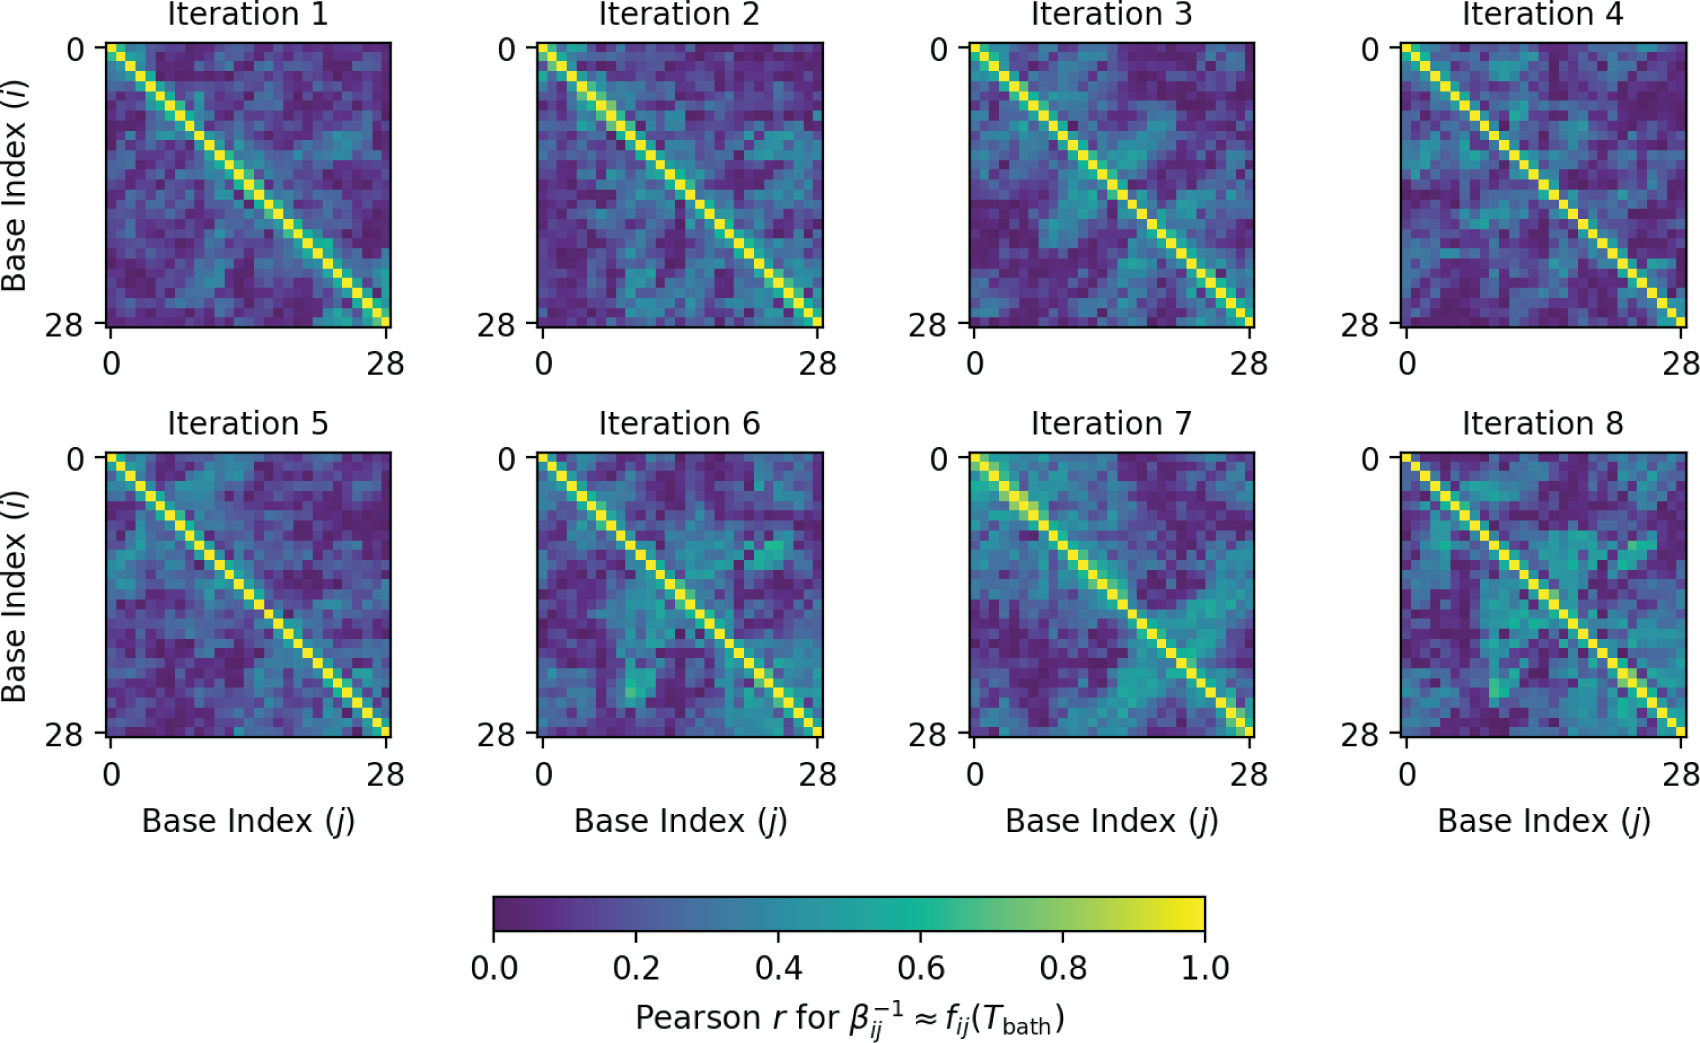
\includegraphics[
    width=0.9\textwidth
    ]{figures/ch4_si_Fluctuation-mapping-fit.png}
    \caption[Quality of linear fluctuation fit for the HIV-TAR RNA.]{{\bf Quality of linear fluctuation fit for the HIV-TAR RNA.} For each iteration of TM-aMD applied to the HIV-TAR RNA in Section \ref{ch4:sec:RNA} the accuracy of the Fluctuation Mapping method is assessed. Since the dependence of fluctuations with temperature is linear in the prior system we expect that as TM-aMD progresses a similar dependence should be observed in the simulated RNA system. For each iteration of TM-aMD we compute fluctuations from the pairwise displacement vectors $\mathbf{r}$ as $\{\beta_{ij}^{(n)}\}_{n=1}^N = \{ \langle \mathrm{Variance}(\mathbf{r}_{ijk}^{(n)})\rangle_{k}\}_{n=1}^N$, where $i$ and $j$ are nucleobase indices, $k$ denotes the spatial coordinates, and $n$ denotes the replica index. We then evaluate the multilinear fit $\mathbf{f}(T)$, where each $f_{ij}$ is a linear fit to $\{(T^{(n)},{\beta^{(n)}_{ij}}^{-1})\}_{n=1}^{N}$. The quality of the fit, and therefore the validity of the Fluctuation Mapping assumption, is characterized by the Pearson $r$ values for each $f_{ij}$, as depicted in the figure. Initially, the assumption is inaccurate, as evidenced by the number of entries with small $r$ values. However, as more iterations of TM-aMD are performed the quality of fit improves, indicating the thermodynamics of the replica simulations more closely matches that of the prior, validating our use of Fluctuation Mapping.}
    \label{ch4:fig:fluctuation-mapping-fit}
\end{figure}

\begin{figure}[p]
    \centering
    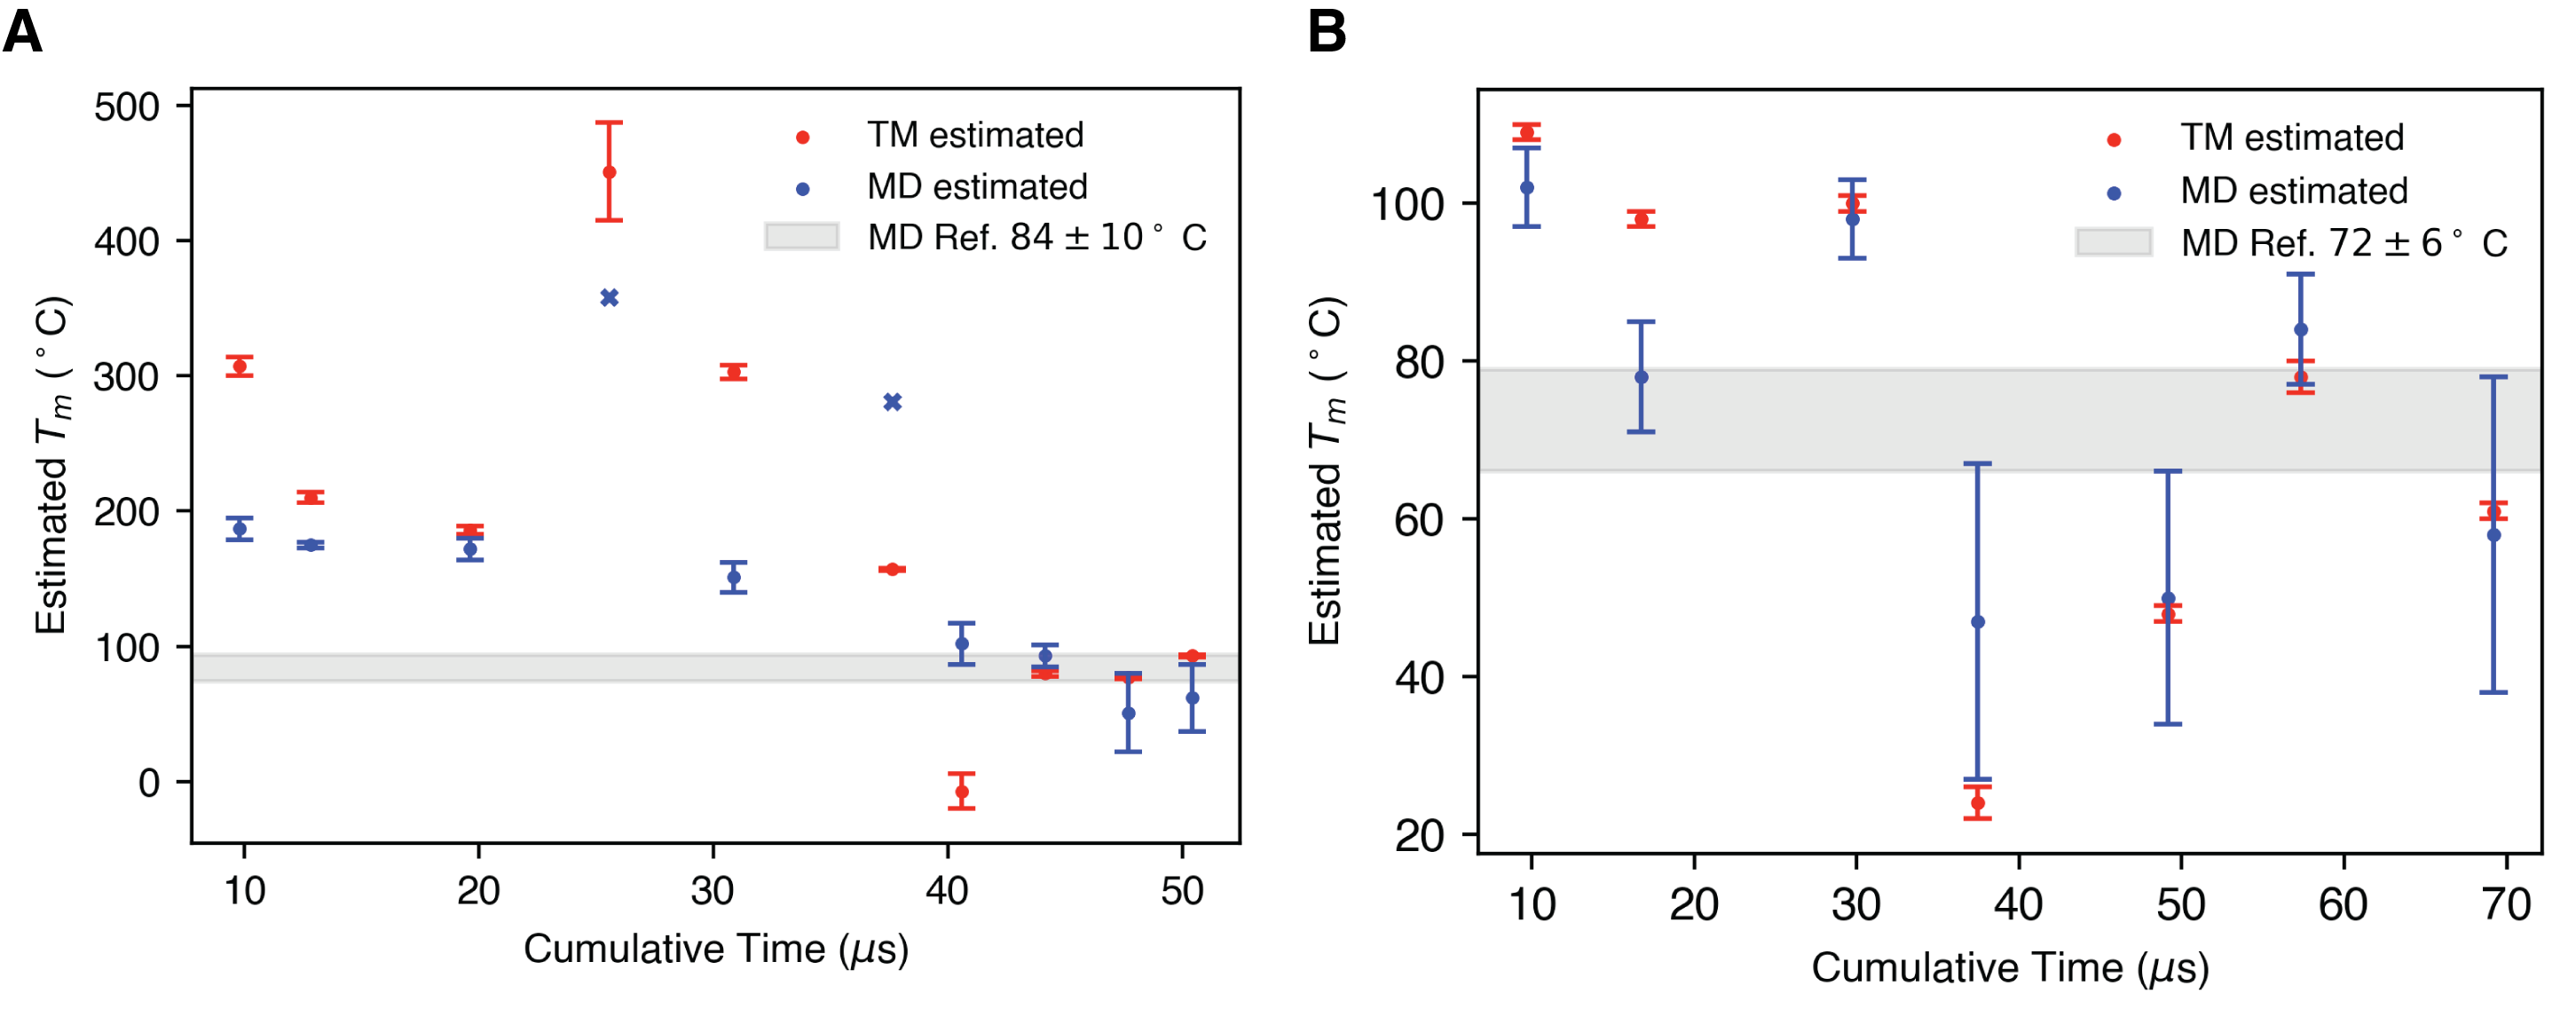
\includegraphics[
    width=\textwidth
    ]{figures/ch4_si_Figure-convergence.png}
    \caption[Convergence of melting temperature calculations.]{{\bf Convergence of Melting Temperature Calculations.} {\bf A} Melting temperatures for the GCAA tetraloop computed independently for each iteration of TM-aMD with one standard deviation uncertainties on the prediction. Convergence occurs after 45$\mu$s of MD simulation. For visual clarity, predictions with uncertainties greater than 100$^\circ$C are represented as x's. {\bf B} Melting temperatures for HIV-TAR are computed independently for each iteration of TM-aMD with one standard deviation uncertainties on the prediction. In both panels, the TM predictions show smaller uncertainties relative to the MD predictions.}
    \label{ch4:fig:convergence}
\end{figure}

\begin{figure}[p]
    \centering
    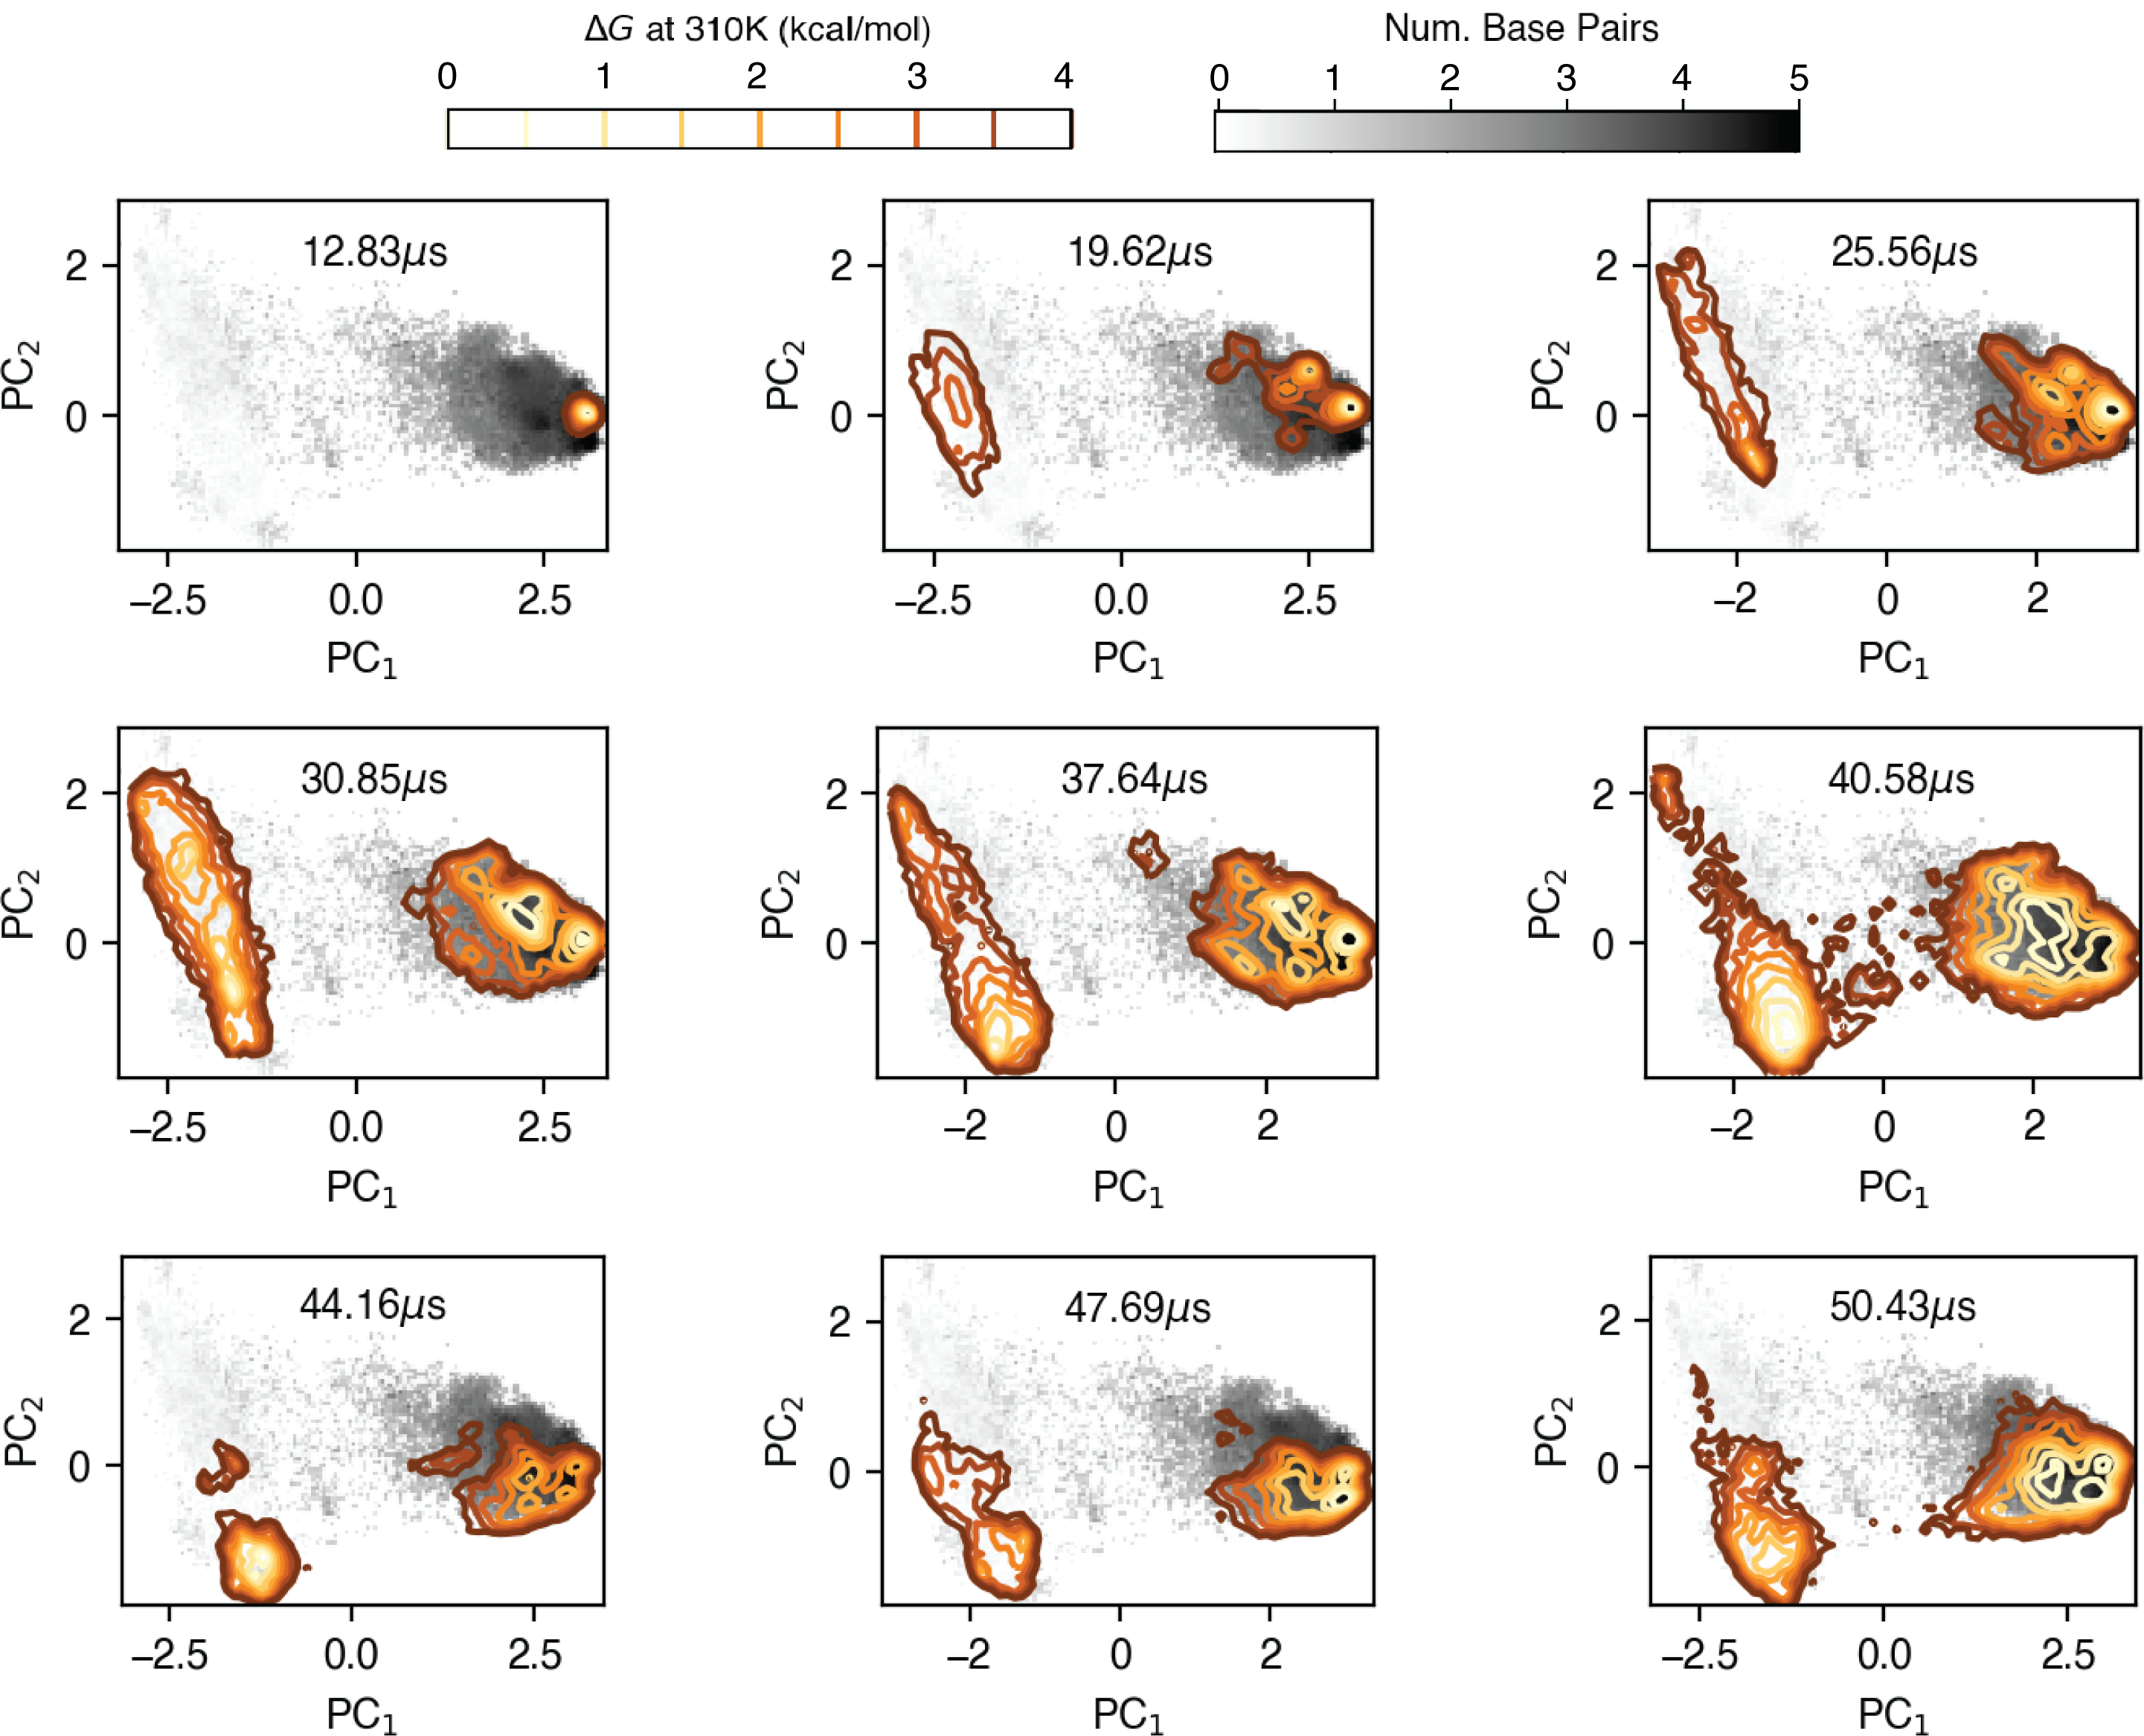
\includegraphics[
    width=\textwidth
    ]{figures/ch4_si_Figure-gcaa-contour-series.png}
    \caption[Convergence towards equilibrium for GCAA.]{{\bf Convergence Towards Equilibrium for GCAA.} The TM-predicted conformational landscape at each iteration is superimposed on the distribution of all MD structures, shaded by the number of base pairs. The cumulative simulation time associated with iteration is listed.}
    \label{ch4:fig:gcaa-contours}
\end{figure}

\begin{figure}[p]
    \centering
    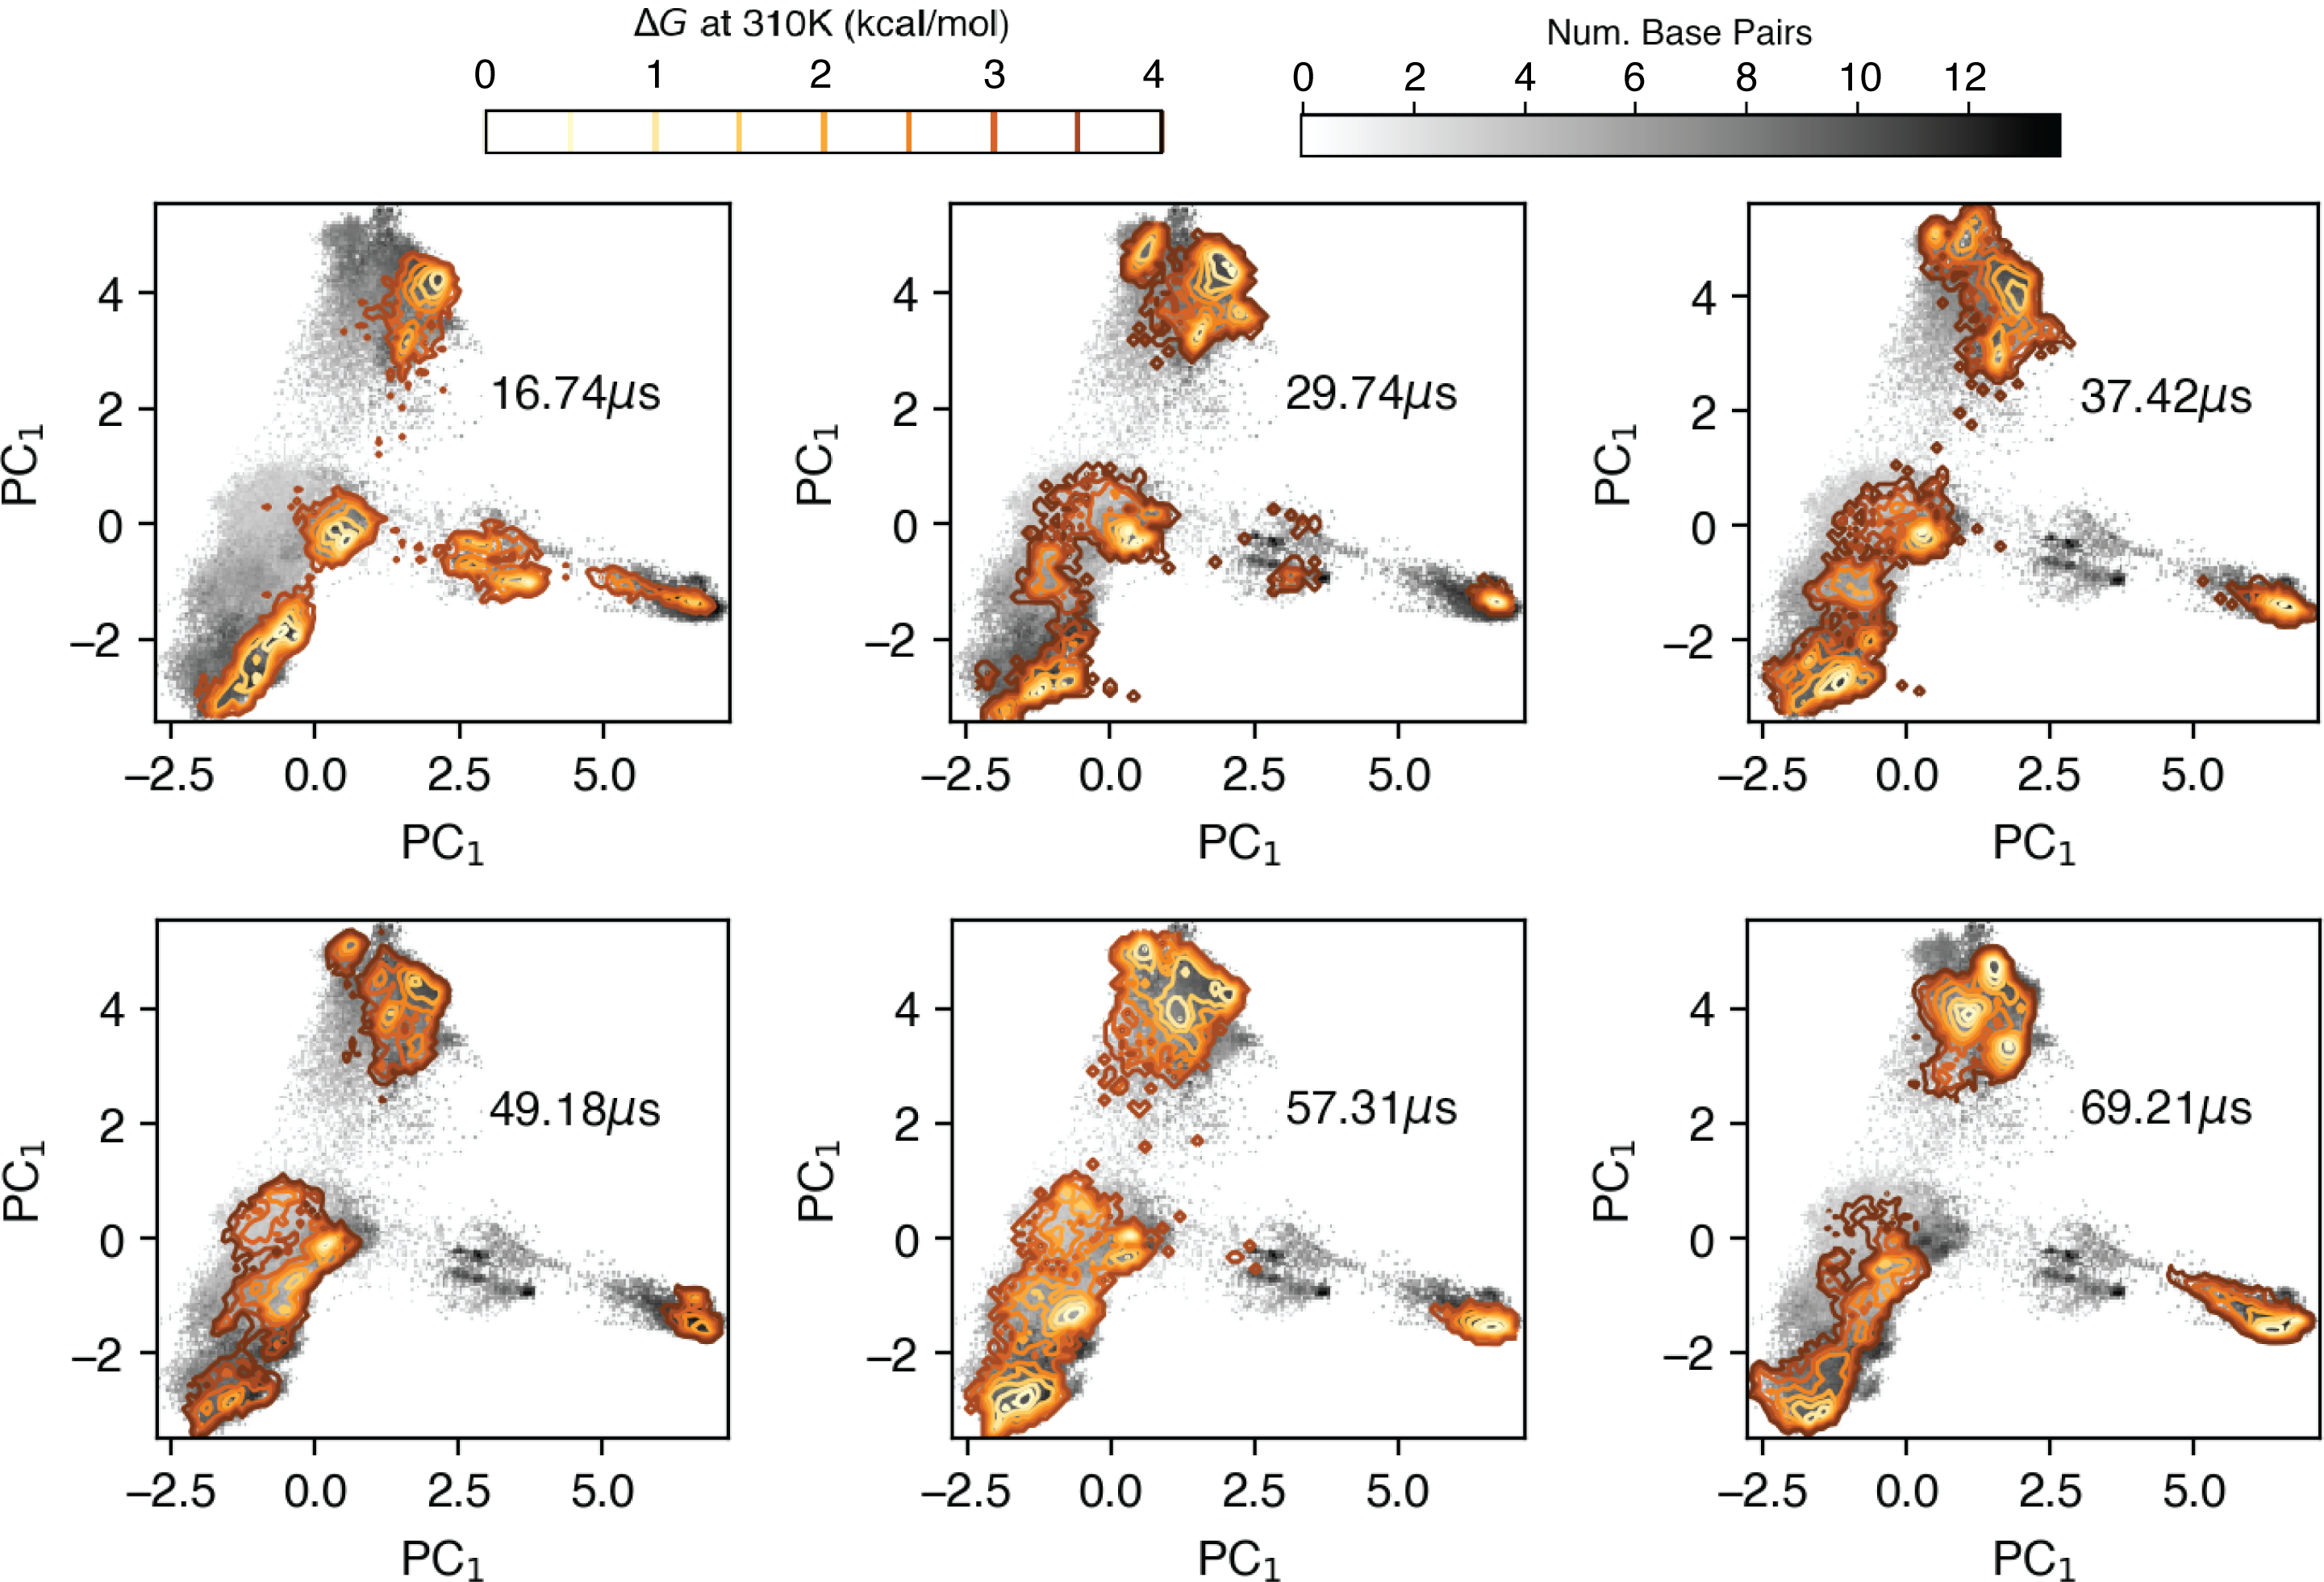
\includegraphics[
    width=\textwidth
    ]{figures/ch4_si_Figure-hiv-tar-contour-series.png}
    \caption[Convergence towards equilibrium for HIV-TAR.]{{\bf Convergence Towards Equilibrium for HIV-TAR.} The TM-predicted conformational landscape at each iteration is superimposed on the distribution of all MD structures, shaded by the number of base pairs. The cumulative simulation time associated with iteration is listed.}
    \label{ch4:fig:hiv-tar-contours}
\end{figure}
